\documentclass{newlayout}
%Bitte hier den enstprechenden Ort einsetzen z.B. Braunschweig und die Akademienummer
\Akademie{Rossleben}{2017}{5}

\usepackage[ngerman,english]{babel}
\usepackage{misc}
\usepackage{multicol}
\usepackage{booktabs}

\usepackage{color}% für Farben im allgemeinen
\usepackage{colortbl}

\usepackage{url}
\usepackage{breakurl}

\usepackage{units}

% hinzugef?gt, um Fehler 'pdfTeX error (font expansion): auto expansion is only possible with scalable' zu vermeiden
%\usepackage{lmodern}
\setkomafont{descriptionlabel}{\normalfont\bfseries}
\addtokomafont{paragraph}{\normalfont}
\usepackage{footnote}
\usepackage[flushmargin,hang,ragged]{footmisc}
\deffootnote{1em}{1em}{%
\textsuperscript{\thefootnotemark\ }
}

%\usepackage{amsmath}%wird automatisch durch newlayout.cls geladen
\usepackage{amsfonts}

%%%%%Mathe-Definitionen
\newtheorem{Def}{Definition}
\newtheorem{Sat}{Satz}
\newtheorem{Bew}{Beweis}

\setlength\abovedisplayshortskip{0pt}
\setlength\belowdisplayshortskip{0pt}
\setlength\abovedisplayskip{3pt}
\setlength\belowdisplayskip{3pt}
%%%%Ende Mathe-Definitionen

\begin{document}

 %   \input{titel}
 \setcounter{page}{3}

\setcounter{tocdepth}{1}
 \tableofcontents

   \setcounter{secnumdepth}{1}


\setcounter{page}{7}
\setcounter{chapter}{0}

%Angabe, bis zu welcher Stufe die sections im Text nummeriert werden sollen.
      \settocdepth{2}

\graphicspath{ {./pics/} }


\course{1}{Die Farbe Blau}%%% 
\begin{coursetitle}
  \centerline{Die Farbe Blau} 
  \bigskip
  %\Large \centerline{Kursuntertitel eingeben}
  \bigskip
 %\includegraphics[width=.9\textwidth]{kurslogo.png}
 \label{fig:meinbild}
  \bigskip
\end{coursetitle}


%\section{Gasentladung}

\section{Die Schrödingergleichung}
\authors{Lena Trahe, Lynn Meeder}

Um die Struktur, Energie und Eigenschaften von Atomen und Molekülen zu beschreiben, bedient man sich der Quantenmechanik \cite{Reinhold}.

\subsection{Operatoren und Eigenwertprobleme}

Wendet man einen Operator $\hat{A}$ auf eine Funktion $f(x)$ an, so erhält man eine neue Funktion $g(x)$. Ein bekannter Operator ist zum Beispiel der Differentialoperator  $\frac{d}{dx}$.

Für einen solchen Operator lässt sich eine Eigenwertproblem formulieren, in dem $g(x)= af(x)$ und somit folgende Gleichung gilt:

\begin{equation}
\hat{A}f(x)=af(x)
 \label{OperatorEigenwert}
\end{equation}

Gesucht sind nun die Eigenfunktionen $f(x)$ und die Eigenwerte a, die Gleichung \ref{OperatorEigenwert} genügen.

\subsection{Zeitunabhängige Schrödingergleichung}

Die zeitunabhängige Schrödingergleichung ist das Eigenwertproblem des Hamilton-Operators $\hat{H}$:

\begin{equation}
\hat{H} \psi = E \psi
\end{equation}

Der Hamilton-Operator ist der Operator der Gesamtenergie $E$. Die Gesamtenergie ist die Summe aus kinetischer Energie $T$, die vom Impuls $\vec{p}$ abhängt, und potentieller Energie $V$, die vom Ort $\vec{x}$ abhängt. Analog ist der Hamilton-Operator die Summe aus den Operatoren für die kinetische und die potentielle Energie:

\begin{equation}
\hat{H}(\hat{\vec{p}}, \hat{\vec{x}}) = \hat{T} (\hat{\vec{p}}) + \hat{V} (\hat{\vec{x}})
\label{HamiltonOperatorTV}
\end{equation}

$\hat{\vec{p}}$ ist somit der Impulsoperator und $\hat{\vec{x}}$ der Ortsoperator. Die kinetische Energie $T$ wird in der klassischen Mechanik als $\frac{\vec{p}^2}{2m}$ beschrieben. Den Impulsoperator $\hat{\vec{p}}$ stellt man in der Quantenmechanik nun dar als 

\begin{equation}
\hat{\vec{p}} = -i\hbar \left( 
\begin{array}{c}
\frac{\partial}{\partial x} \\ \frac{\partial}{\partial y} \\ \frac{\partial}{\partial z}
\end{array} \right)
\end{equation}

Durch Einsetzen in den Ausdruck $\hat{T}=\frac{\hat{\vec{p}}^2}{2m}$ erhält man:

\begin{equation}
\hat{T}=-\frac{\hbar^2}{2m}  \left( \frac{\partial ^2}{\partial  x^2}+\frac{\partial ^2}{\partial  y^2}+\frac{\partial ^2}{\partial  z^2}\right)
\end{equation}

Die potentielle Energie hängt nur vom Ort $\vec{x}$ ab und ist deshalb in der Ortsdarstellung ein multiplikativer Operator: $\hat{V}(\hat{x})=\hat{V}(x)$. Die potentielle Energie eines Elektrons mit der Ladung $-e$ im Feld eines Protons mit der Ladung $+e$ beträgt $\hat{V}(x) = -\frac{1}{4 \pi \epsilon_0}\frac{e^2}{r}$. r bezeichnet die Entfernung des Elektrons zum Kern. Für das Wasserstoffatom lautet Gleichung \ref{HamiltonOperatorTV} also:

\begin{equation}
\left[ - \frac{\hbar^2}{2m}  \hat{\vec{\nabla}}^2 -\frac{1}{4 \pi \epsilon_0}\frac{e^2}{r} \right] \psi = E\psi
\end{equation}

Wobei der Operator $\hat{\vec{\nabla}}^2$ gegeben ist als:

\begin{equation}
\hat{\vec{\nabla}}^2 = \frac{\partial ^2}{\partial  x^2}+\frac{\partial ^2}{\partial  y^2}+\frac{\partial ^2}{\partial  z^2}
\end{equation}

Die diskreten Energieeigenwerte $E$ sind hier:

\begin{equation}
E_n=-\frac{m_e e^4}{2\hbar^2}\frac{1}{n^2} \:mit \: n\in \mathbb{N}
\end{equation}

\section{Hückeltheorie}

Autoren: David Bürg, Isabelle Schulte-Herbrüggen

Die Hückeltheorie wurde in den 1930er Jahren von Erick Hückel entwickelt. \cite{Reinhold} Sie erlaubt eine einfache Beschreibung von konjugierten Doppelbindungssystemen. Die Methode arbeitet mit vielen Näherungen. Daher ist sie zwar ungenau, aber einfach anzuwenden. Sie baut auf der Näherung von $\pi$-Molekülorbitalen und deren Energien über Linearkombinationen von p-Atomorbitalen auf. Die Linearkombinationen können mit:

\begin{align}
 \psi_{i} = \sum \limits_{k=1}^n c_{ik} \chi_k 
\end{align}

beschrieben werden. Der Koeffizient $c_{ik}$ gibt hierbei an, wie  stark die einzelnen Atomorbitale $\chi_k$ am Molekülorbital $\psi_i$ beteiligt sind. Die Koeffizienten $c_{ik}$ lassen sich über die Summen:

\begin{align}\label{eq:hueckel}
  \sum \limits_{k=1}^n (H_{jk}-\epsilon_i S_{jk}) c_{ik} = 0
\end{align}

bestimmen. $H_{jk}$ ist das Hamiltonmatrixelement, $S_{jk}$ das Überlappmatrixselement und $\epsilon_i$ ist die Energie des Molekülorbitals. Mit Gleichung (\ref{eq:hueckel}) kann nun die Hückelmatrix formuliert werden. Dabei wird angenommen, dass die Hamiltonmatrixelemente aller Kohlenstoffatome gleich sind, sowie dass die Wechselwirkungen aller nächsten Nachbarn gleich sind. Zusätzlich vereinfacht man die Beschreibung noch weiter, indem die Wechselwirkungen zwischen nicht-nächsten Nachbarn komplett vernachlässigt werden. Aufgrund dieser Vereinfachungen sind die Ergebnisse, die man durch Anwenden der Hückeltheorie erhält, grobe Näherungen.


Indem man fordert, dass die Determinante der Hückelmatrix verschwindet, erhält man einen Satz gekoppelter Gleichungen, deren Lösung die Koeffizienten $c_{ik}$ und die Orbitalenergien $\epsilon_i$ liefert. So kann nun die Energiedifferenz zwischen HOMO und LUMO mit:

\begin{align}
  \Delta E = \epsilon_{LUMO} - \epsilon_{HOMO}
\end{align}

berechnet werden. Diese Energiedifferenz erlaubt eine grobe Abschätzung der ersten Anregungsenergie des Moleküls.

Beschreibt man das 1,3-Butadien-Molekül mit der Hückelthoerie, erhält man die in Abbildung  \ref{fig:Hueckel_Butadiene} dargestellten Molekülorbitale.

\begin{dsafigure}
 \centering
 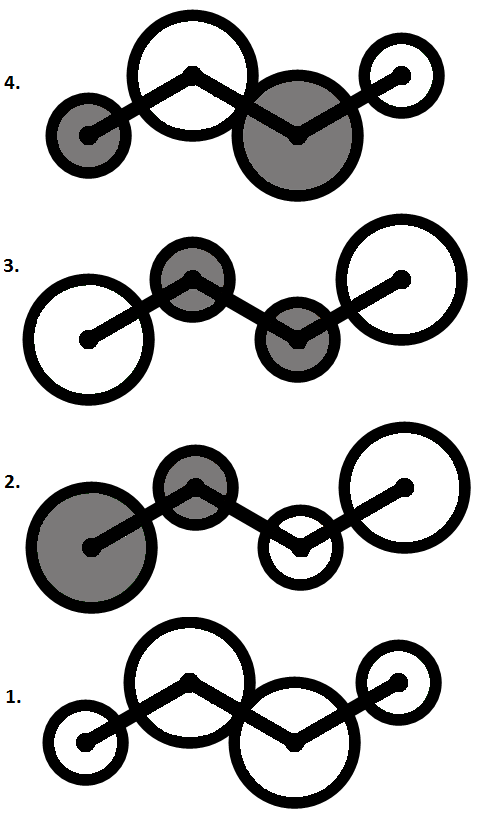
\includegraphics[width=8cm]{Hueckel_Butadiene.png}
 \caption{Aufsicht auf ein 1,3-Butadienmolekül. Schematische Darstellung der Hückelmolekülorbitale von 1,3-Butadien.}
 \label{fig:Hueckel_Butadiene}
\end{dsafigure}

Die Radien der Kreise entsprechen den Koeffizienten $c_{ik}$, während Weiß und Grau die Positivteile beziehungsweise Negativteile beschreiben. Das erste Orbital ist das energetisch günstigste Molekülorbital von Butadien, da es nur bindende Wechselwirkungen aufweist und keine Knotenebene besitzt; es ist ein bindendes Orbital. Das zweite Orbital hingegen weist zwei bindende Wechselwirkungen und eine Knotenebene auf. Es handelt sich auch hier um ein bindendes Orbital. Beim dritten un vierten Orbital handelt es sich um antibindende Orbitale. Das dritte Orbital zeigt zwei Knotenebenen und eine bindende Wechselwirkung und das vierte Orbital weist drei Knotenebenen und keine bindenden Wechselwirkungen auf. Sie haben also mehr Knotenebenen als bindende Wechselwirkungen. Die Energie vier Molekülorbitale nimmt in aufsteigender Reihenfolge zu.

\section{Phosphoreszenz}
\authors{Selin Güler, Joes Biburger}

Mit Phosphoreszenz wird die Emission von Licht bezeichnet, die auf einen Übergang von einem angeregten Triplett- in einen Singulett-Grundzustand zurückzuführen ist. 

Der Phosphoreszenzvorgang beginnt mit der Absorption eines Photons mit spezifischer Wellenlänge durch ein Molekül. Letzteres wird vom Grundzustand in einen angeregten Singulettzustand $(S_1)$, in dem alle Elektronen mit entgegengesetztem Spin gepaart sind, angeregt. Nun erfolgt der als Intersystem Crossing bezeichnete Übergang in einen angeregten Triplettzustand $(T_1)$. In diesem gibt es zwei ungepaarte Elektronen mit gleichem Spin. Der angeregte Triplettzustand $(T_1)$ ist energieärmer und somit stabiler als der angeregte Singulettzustand $(S_1)$. Aufgrund der Tatsache, dass die für den Übergang in den Grundzustand $(S_0)$ notwendige Spinumkehr spinverboten und somit unwahrscheinlich ist, können mehrere Stunden vergehen, bevor das Molekül in den Grundzustand zurückfällt. Bei einem solchen Übergang wird Energie in Form von Licht abgegeben. Das emittierte Licht ist immer langwelliger als das bei der Anregung aufgenommene. Das rührt daher, dass bei der Phosphoreszenz, ähnlich wie bei der Fluoreszenz, verschiedene Schwingungszustände innerhalb des Grund- $(S_0)$ sowie angeregten Triplettzustandes $(T_1)$ existieren. Das Molekül gibt beim Übergehen in den energieärmsten Schwingungszustand Energie strahlungsfrei an weitere Translations-, Rotations-, Schwingungsmoden ab, weshalb nur ein Teil der Energie des absorbierten Lichtes in Form von Licht wieder emittiert wird. 
\cite{Phosphoreszenz1}, \cite{Phosphoreszenz2}, \cite{Phosphoreszenz3}



\section*{Literaturverzeichnis}
\bibliographystyle{jcpsty_deutsch}
%\bibliographystyle{unsrtdin}
\bibliography{lit2}

\end{document}
